\section{Core System Modules}
The following modules are included in RTXI by default and are available through the \textbf{System} menu. No additional modules are necessary for acquiring data through a DAQ card and saving data to an HDF5 file.

\subsection{System Control Panel}
\label{system control panel}
\index{System Control Panel}

The System Control Panel allows you to set important parameters on all the input and output channels of your DAQ card and set the nominal real-time period of your system. RTXI automatically detects the manufacturer and board names of available DAQ cards and the number and type of input and output channels. The first DAQ card installed in your system is assigned the Linux device name: \texttt{/dev/comedi0}. \seealso{Chapter \ref{more DAQ cards}\\Configure RTXI for more cards}Additional DAQ cards are assigned device names \texttt{/dev/comedi1} and so on.

\begin{figure}[h]
\begin{center}
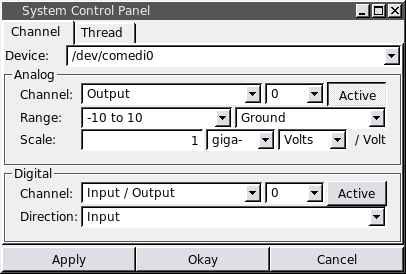
\includegraphics[width=4.5in]{systemcontrol0.png} 
\caption[System Control Panel: Channel Tab]{The Channel Tab allows users to activate and set channel properties on the DAQ card.} 
\end{center}
\label{fig:systemcontrolpanel0}
\end{figure}

\marginlabel{Channel Tab}\index{DAQ, configuration}By default, RTXI assumes that all analog DAQ input and output channels have a range from -10 V to +10 V, unity gain (or a scaling of 1 V/V), and a ground reference. You must set the correct options for each channel you are using to acquire and output the correct signal values. In the screenshot below, the DAQ card is being used as a signal generator on the first analog output channel (Channel 0). This channel is connected to an external amplifier that specifies a gain of 1 nA/V. This gain is inverted here to 1 gigaVolt/Volt to output the correct values and can be verified on an external oscilloscope. For your own reference, you could set the dropdown boxes to read 1 gigaAmp/Volt to indicate that you are ultimately generating a current signal, but this setting does not affect the computation. \attention You must click the \textbf{``Active"} toggle button to actually activate the channel. You must click \textbf{``Apply"} to commit changes made to any other channel properties such as the scale. When you have set the correct parameters for all your input and output channels, you can save your settings by choosing \textbf{File}$\rightarrow$\textbf{Save Workspace} from the RTXI menu bar. This will create a basic *.set file that you can load in the future to recreate this environment or use as a foundation for additional *.set files.

\marginlabel{Thread Tab}\index{real-time period}\index{sampling rate}In the Thread tab, you can change the real-time period of the entire system. You must click ``Apply" for this change to take effect because it triggers a real-time event that is propagated to other modules. \seealso{Chapter \ref{pause flag}\\\texttt{DefaultGUIModel} PAUSE flag}Custom user modules can be programmed to execute specific code when the system's real-time period is changed.

\begin{figure}[h]
\begin{center}
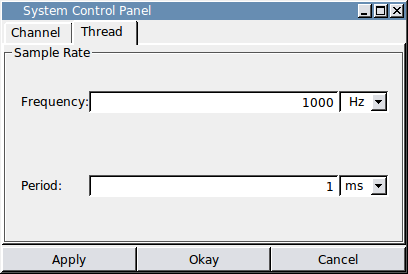
\includegraphics[width=4.5in]{systemcontrol1.png} 
\caption[System Control Panel: Thread Tab]{The Thread Tab allows users to change the period for real-time execution.} 
\end{center}
\label{fig:systemcontrolpanel1}
\end{figure}

\subsection{Oscilloscope}
\label{Oscilloscope}
\index{Oscilloscope}

The Oscilloscope allows you to plot any system signal in real-time, including signals from/to the DAQ card and signals from user modules. To plot multiple signals, you can instantiate multiple oscilloscopes or superimpose multiple signals on a single oscilloscope. Each signal may have a different vertical scale and line style and a legend is automatically generated in the Oscilloscope window. Below is a screenshot of the Oscilloscope acquiring data using the CLAMP-1U model cell (by Molecular Devices) with an applied square pulse current. It is plotting two input channels from the DAQ card as well as the command current (Iout1) generated by a module. The lower right-hand corner displays the time scale for each grid division. \attention The Oscilloscope uses a right-click context menu that allows you to pause/unpause real-time plotting or access the ``Properties" panel for choosing signals and setting the axes properties.

\begin{figure}[h]
\begin{maxipage}
\begin{center}
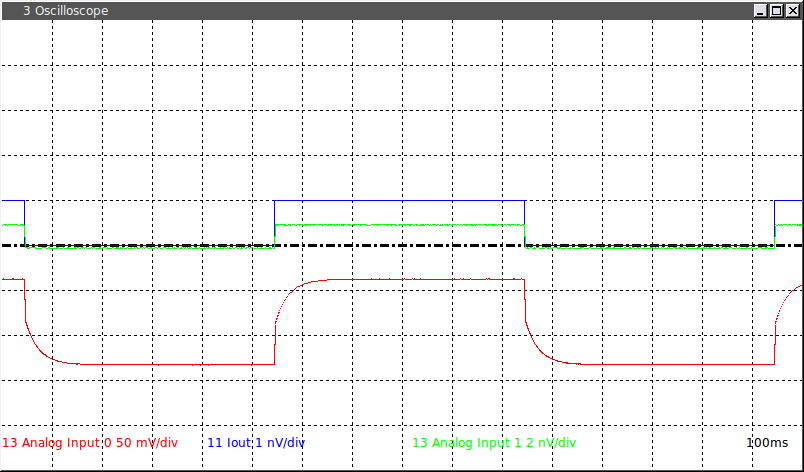
\includegraphics[width=6in]{oscilloscope0.png} 
\caption[Oscilloscope]{The Oscilloscope can plot multiple signals in real-time.} 
\end{center}
\label{fig:oscilloscopel0}
\end{maxipage}
\end{figure}

\marginlabel{Channel Tab}On the Channel tab, you can select signals to plot. Signals from the DAQ card will appear in the ``�Channel" dropdown box as a COMEDI source, eg. \texttt{/dev/comedi0}. To get correct values for your signal, you may have to set additional settings in the \seealso{Chapter \ref{system control panel}\\System Control Panel}System Control panel if you use any other instrumentation that applies a gain to your signal. Input to the DAQ card from external instrumentation, such as an external amplifier, is designated as output from the DAQ card within RTXI. RTXI will automatically detect how many input and output channels your card has. Signals from other modules will be identified by the module name and you can choose from any inputs, outputs, parameters, or states that are defined in those modules. \attention To actually plot the signal, you must depress the \textbf{``Active"} toggle button and hit \textbf{``Apply."} Any modifications you make to the scaling, offset, or line style of the signal are not active until you hit ``Apply" again. Note that plotting too many signals in real-time may affect your system performance and cause your GUI to freeze during program execution.

\begin{figure}[h]
\begin{center}
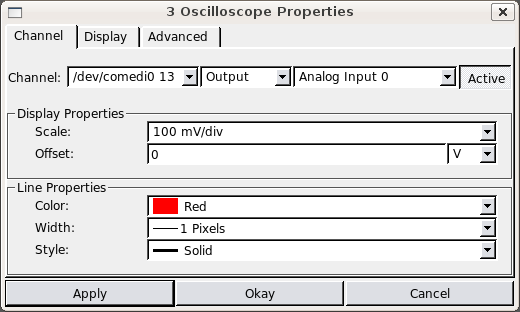
\includegraphics[width=4.5in]{oscilloscope1.png} 
\caption[Oscilloscope: Channel Tab]{The Channel Tab allows you to select the signals to plot and set line styles.} 
\end{center}
\label{fig:oscilloscope1}
\end{figure}

\newpage
\marginlabel{Display Tab}On the Display tab, you can set the time scale of the oscilloscope and the screen�s refresh rate. You can also set up a trigger to freeze the oscilloscope when certain criteria are met by the triggered channel. \index{Oscilloscope, trigger}Set the trigger to operate on a ``rising edge" or ``falling edge" by clicking the radio buttons marked ``+" or ``-", respectively. The ``Trigger Channel" can be set to any signal that is currently plotted on the oscilloscope. ``Trigger holding" allows you to set the amount of time that lapses before the trigger is reset again. The trigger threshold is indicated on the oscilloscope by a horizontal yellow dashed line.

\begin{figure}[h!]
\begin{center}
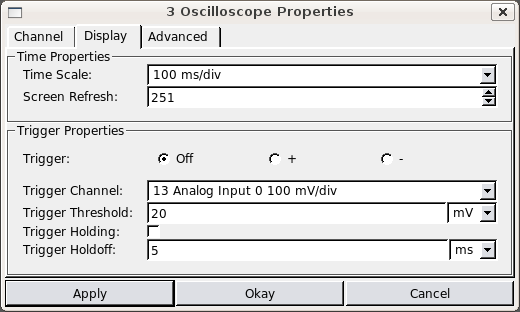
\includegraphics[width=4.5in]{oscilloscope2.png} 
\caption[Oscilloscope: Display Tab]{The Display Tab allows you to set the time scale for horizontal divisions and set a trigger on any plotted signal.} 
\end{center}
\label{fig:oscilloscope2}
\end{figure}

\newpage
\marginlabel{Advanced Tab}On the Advanced tab, you can choose to downsample the data that is plotted on the oscilloscope or change the number of grid divisions used for scaling.

\begin{figure}[h]
\begin{center}
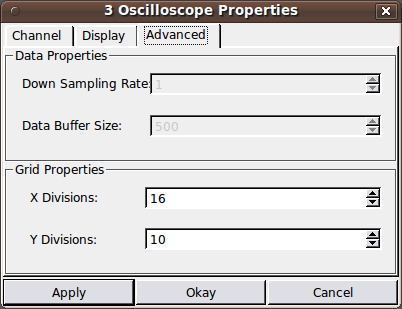
\includegraphics[width=4in]{oscilloscope3.png} 
\caption[Oscilloscope: Advanced Tab]{The Advanced Tab allows users to set downsampling rates on the plotted data, change the size of the data buffer, and change the number of divisions in the oscilloscope.} 
\end{center}
\label{fig:oscilloscope3}
\end{figure}

\subsection{Data Recorder}
\index{Data Recorder}

The Data Recorder module allows users to stream synchronous data to a HDF5 file. To record data, select \textbf{System}$\rightarrow$\textbf{Data Recorder} from the RTXI menu bar. The \textbf{``Block"} menu is a list of your DAQ card(s) and any loaded user modules. Selecting a block device then populates the \textbf{``Type"} and \textbf{``Channel"} menus. Select the Analog Input 0 channel from your DAQ device and click the \textbf{``$>$"} button. To remove a channel from the list, highlight it in the listbox and click the \textbf{``$<$"} button. Before you can start recording, you must select a file by clicking the \textbf{``Choose File"} button. Click \textbf{``Start Recording"} to begin recording and \textbf{``Stop Recording"} to stop recording. For each module connected to the Data Recorder, it also grabs all the parameters values and saves them as metadata. In addition, it logs when any of these parameter values change so that you have a complete record of your experiment. If you have a configuration such that Module A: Output 0 --$>$ Module B: Input 0, saving both of these respective signals in the Data Recorder will give you exactly the same data. Similarly, saving \texttt{/dev/comedi0}: Analog Output 0 will save the signal that has been assigned to that channel (perhaps generated by a user module), not the actual signal the DAQ card is outputting. To check the actual output of the DAQ card, you will need to make a connection from that output to another input channel.

\begin{figure}[h]
\begin{center}
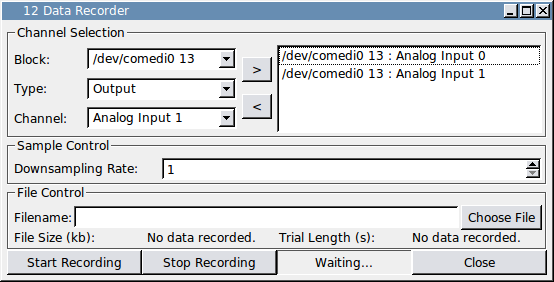
\includegraphics[width=4.5in]{datarecorder.png} 
\caption[Data Recorder]{The Data Recorder allows you to save any signal in your workspace synchronously to an HDF5 file. Use the  ``$>$" and ``$<$" buttons to add and remove signals from the list.} 
\end{center}
\label{fig:datarecorder}
\end{figure}

For real-time streaming of multiple signals, an HDF5 data type is used in RTXI that does not map efficiently onto MATLAB native data types. While MATLAB can read this data using its low-level functions, this process can be very slow. To load RTXI HDF5 files quickly into MATLAB, you will first need to run a small utility function on your HDF5 file to convert the \emph{Synchronous Data} dataset to a different data type. This function is compiled when RTXI is compiled and is located in \texttt{/rtxi/hdf}. To convert your HDF5 file:\index{rtxi\_hdf\_matlabize}
\begin{example}
\$ rtxi\_hdf\_matlablize YOUR\_FILE.h5
\end{example}

To make this utility accessible from any directory on your system, make a symbolic link in \texttt{/usr/bin} to the location of this function in your RTXI source directory. If you installed RTXI from the Live CD, the source directory is \texttt{/home/rtxi}:
\begin{example}
\$ sudo ln -s RTXI\_SRC\_DIR/hdf/rtxi\_hdf\_matlabize \\ \hspace{1cm} /usr/bin/rtxi\_hdf\_matlabize
\end{example}

RTXI also includes a simple MATLAB GUI for quickly viewing the data within a single trial. The MATLAB code is available in \texttt{/rtxi/hdf/RTXIh5}. A sample m-file is provided with examples of how to extract data to the MATLAB workspace, how to use the GUI browser, and how to add new datasets to your file. It is also possible to embed binary formats, such as images, within a trial.

\subsection{Connector}
\label{Connector}
\index{Connector}

The Connector module allows you to create connections between modules or between modules and the DAQ card. Incoming signals to RTXI through the DAQ card appear in the \textbf{``Output Block"} and outgoing signals through the DAQ appear in the \textbf{``Input Block."} RTXI automatically detects how many inputs and outputs are available for your installed DAQ card. Similarly, any signal that is defined as an output of a module appears in the ``Output Block" and any input slot of a module appears in the ``Input Block." After you have made your selection, click the central toggle button to activate the connection. Your active connections are listed in the ``Connections" box. To quickly turn off an existing connection, double-click on its entry in the table and click the toggle button. Below is a screenshot of how to connect the command current from the Istep module to the first analog output channel of the DAQ card.

\begin{figure}[h]
\begin{center}
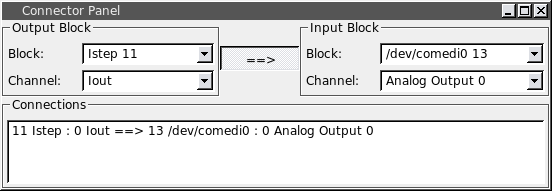
\includegraphics[width=4.5in]{connector1.png} 
\caption[Connector]{The Connector allows you to connect any signal from the left ``Output Block" and connect it to a slot in the right ``Input Block". RTXI automatically detects the available signals and slots from the DAQ card and any loaded user modules.} 
\end{center}
\label{fig:connector1}
\end{figure}

Here is a screenshot containing connections between modules only. The membrane potential of a model neuron is fed into a spike detector that in turn, informs a dynamic clamp module when spikes have occurred. The model cell�s voltage is also fed into the dynamic clamp module for computing the current that is connected back to the model cell. \attention The signals-and-slots architecture of RTXI allows any signal to be connected to any slot. In this example, the spike detector could accept input from any model neuron simulated within RTXI or input from an actual recorded cell. RTXI also allows one-to-many and many-to-one connections. If multiple signals are connected to one slot, the signals are first summed before any additional operations are performed. Thus, multiple signals could be connected to be a single output channel of your DAQ card, allowing you to ``stack" stimuli being generated from multiple user modules.

\begin{figure}[h]
\begin{center}
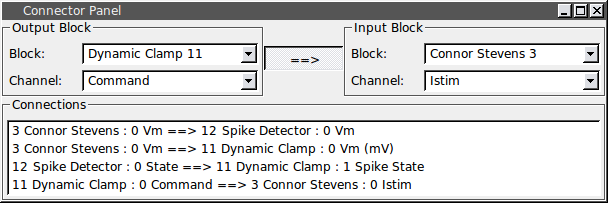
\includegraphics[width=4.5in]{connector.png} 
\caption[Connector]{The signals-and-slots architecture of RTXI allows any signal to be connected to any slot and allows one-to-many and many-to-one connections.} 
\end{center}
\label{fig:connector}
\end{figure}

\subsection{Performance Benchmark}

The Performance Benchmark module gives you timing statistics for RTXI. For hard real-time performance, it is important that all operations, computations executed by user modules and tasks related to data acquisition, etc., complete within the nominal system period. This module continuously keeps track of the time needed to complete these tasks, updated once every second in the GUI, as well as the actual real-time period. In addition, the module reports the worst case total computation time and the worst case time step since the statistics were last reset.

\begin{figure}[h]
\begin{center}
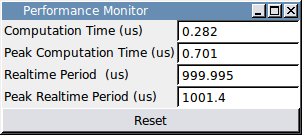
\includegraphics[width=3in]{performancebenchmark0} 
\caption[Performance Benchmark]{The Performance Benchmark module gives you timing statistics related to computational tasks and the actual real-time period (system sampling rate).} 
\end{center}
\label{fig:performancebenchmark0}
\end{figure}